\section{PHÂN TÍCH THIẾT KẾ HỆ THỐNG}

\subsection{Bài toán nghiệp vụ}

Hệ thống hỗ trợ người dùng
hỏi đáp pháp luật Việt Nam,
phân tích tài liệu
và đàm thoại trực tiếp thời gian thực
với trợ lý pháp lý.
Dựa trên Domain Driven Design DDD, bài toán lớn của hệ thống được bóc tách
và phân chia thành các miền phụ (Subdomain)
với mức độ ưu tiên và chức năng riêng biệt như sau:

\begin{figure}[H]
\centering
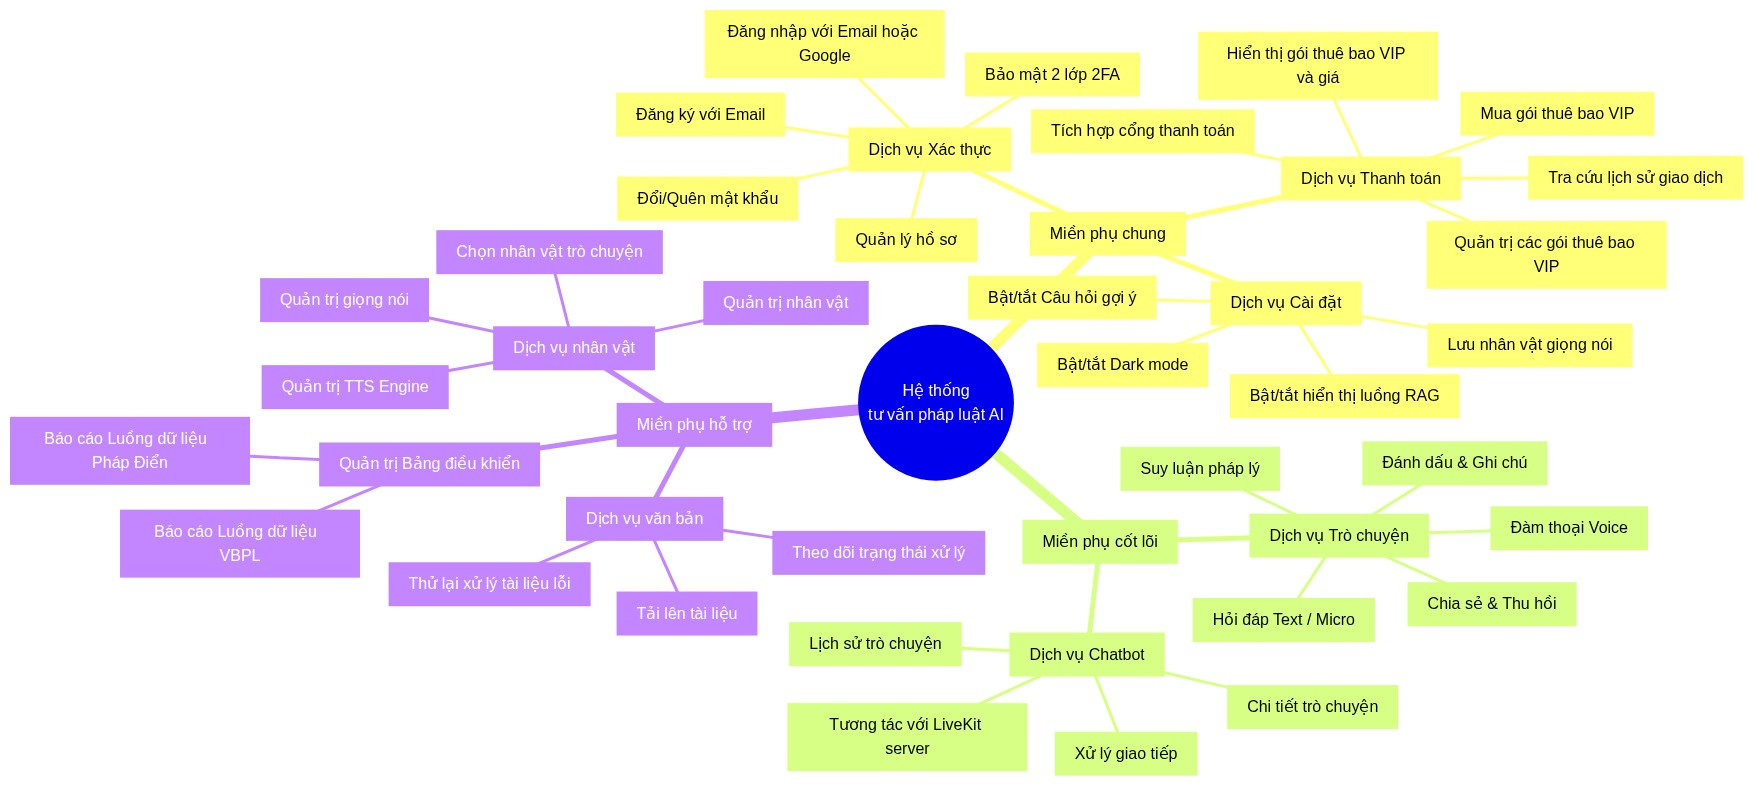
\includegraphics[scale = 0.24]{pictures/SubDomainMindMap.png}
\caption{Sơ đồ tổng quan các miền phụ trong dự án}
\end{figure}

\subsubsection{Miền phụ cốt lõi (Core Subdomain)}

Miền phụ cốt lõi
là phần quan trọng
và có giá trị nhất của hệ thống.
Miền phụ cốt lõi
giúp phân biệt các doanh nghiệp
và làm cho các doanh nghiệp có giá trị.
Miền phụ cốt lõi
tập trung vào mục tiêu
và yêu cầu của khách hàng với doanh nghiệp,
từ đó quyết định sự thành công của doanh nghiệp.
Vì vậy, mỗi doanh nghiệp
luôn tìm cách thực hiện những điều khác biệt
trong các miền phụ cốt lõi này để đạt được lợi thế so với đối thủ cạnh tranh.

% Trong dự án này, miền phụ cốt lõi tập trung giải quyết trực tiếp nhu cầu lớn nhất của người dùng: tra cứu và nhận tư vấn pháp lý chính xác. Mọi tài nguyên, nỗ lực nghiên cứu các thuật toán AI (như RAG, LLM Reasoning) và công sức xây dựng đường ống dữ liệu (Data Pipeline) từ các nguồn luật pháp uy tín đều được dồn vào miền này để đảm bảo câu trả lời đưa ra đạt độ chính xác cao nhất.

\input{contents/SubDomain-Core.tex}

Miền phụ cốt lõi
là nơi diễn ra các luồng xử lý phức tạp
và quyết định đến mức độ hài lòng của người dùng.

\subsubsection{Miền phụ hỗ trợ (Supporting Subdomain)}

% Các miền phụ cốt lõi phụ thuộc
% vào các miền phụ hỗ trợ.
% Miền phụ hỗ trợ cung cấp các dịch vụ
% để miền phụ cốt lõi hoạt động hiệu quả.
% Tuy nhiên, miền phụ hỗ trợ không đòi hỏi mức độ phức tạp cao về logic nghiệp vụ.

Mặc dù miền phụ cốt lõi rất quan trọng, nhưng nó không thể tự mình mang lại một trải nghiệm toàn diện nếu thiếu đi các miền phụ hỗ trợ.
Miền phụ hỗ trợ cung cấp các dịch vụ phụ trợ, bổ sung tính năng để miền phụ cốt lõi hoạt động hiệu quả và thân thiện hơn với người dùng.
Tuy nhiên, các miền này không đòi hỏi mức độ phức tạp quá cao về logic nghiệp vụ.

\begin{itemize}

\item Dịch vụ văn bản (document service)
\begin{itemize}
\item Tải lên file tài liệu văn bản (chỉ dành cho người dùng đã thanh toán VIP)
\item Lấy thông tin trạng thái văn bản
\item Thử lại xử lý tài liệu do bị lỗi
\end{itemize}

\item Dịch vụ nhân vật (persona service)
\begin{itemize}
\item Người dùng lựa chọn nhân vật để trò chuyện giọng nói
\item Quản lý nhân vật (cần vai trò ADMIN)
\item Quản lý TTS Engine (cần vai trò ADMIN)
\item Quản lý giọng nói (Voices) (cần vai trò ADMIN)
\item Đồng bộ giọng nói ElevenLabs (cần vai trò ADMIN)
\end{itemize}

\item Báo cáo luồng dữ liệu
\begin{itemize}
\item Báo cáo thông tin luồng dữ liệu của văn bản pháp luật
\item Báo cáo thông tin luồng dữ liệu của Pháp Điển
\end{itemize}

\end{itemize}


Miền phụ hỗ trợ giúp miền phụ cốt lõi không bị phình to.
Tách nhỏ việc quản lý nhân vật, giọng nói
và quá trình xử lý tài liệu tiêu tốn nhiều tài nguyên hệ thống.
Nhờ có miền phụ hỗ trợ,
việc tiêu tốn tài nguyên hệ thống cho các tác vụ nặng như trích xuất văn bản tài liệu hay tổng hợp giọng nói (TTS) được cô lập, quản lý riêng biệt và có thể mở rộng (scale) độc lập mà không làm ảnh hưởng đến hiệu năng truy vấn pháp luật cốt lõi.

\subsubsection{Miền phụ chung (Generic Subdomain)}

Miền phụ chung
cung cấp các giải pháp có sẵn
mà doanh nghiệp có thể mua, thuê.
Miền phụ chung
có thể được tìm thấy trên nhiều ngành.
Doanh nghiệp không thể đạt được bất kỳ lợi thế cạnh tranh so
với đối thủ bằng cách thực hiện những điều khác biệt trong miền phụ chung.

\input{contents/SubDomain-Generic.tex}

Việc áp dụng các giải pháp chuyên nghiệp có sẵn như hệ thống
quản trị danh tính Supabase (cho Auth) hay Neon Data API
(cho cấu hình Settings) giúp dự án rút ngắn đáng kể thời gian phát triển.
Đặc biệt, việc tận dụng hệ thống xác thực hai yếu tố (2FA) có sẵn từ Supabase là
% điều kiện tiên quyết và
cực kỳ quan trọng để bảo vệ các dữ liệu nhạy cảm của người dùng (như tài liệu hợp đồng cá nhân tải lên hệ thống).

Sơ đồ phân rã chức năng
giúp mô tả các chức năng chính
và phân chia chúng thành các phần nhỏ hơn,
từ đó giúp quản lý
và phát triển hệ thống một cách hiệu quả hơn.
Sơ đồ phân rã chức năng
giúp
giải quyết những vấn đề trong phân chia và kiểm soát chức năng.
Sơ đồ phân rã chức năng dưới đây thể hiện chi tiết
các miền phụ này được triển khai thành các nhóm chức năng cụ thể trong hệ thống:

\begin{figure}[H]
\centering
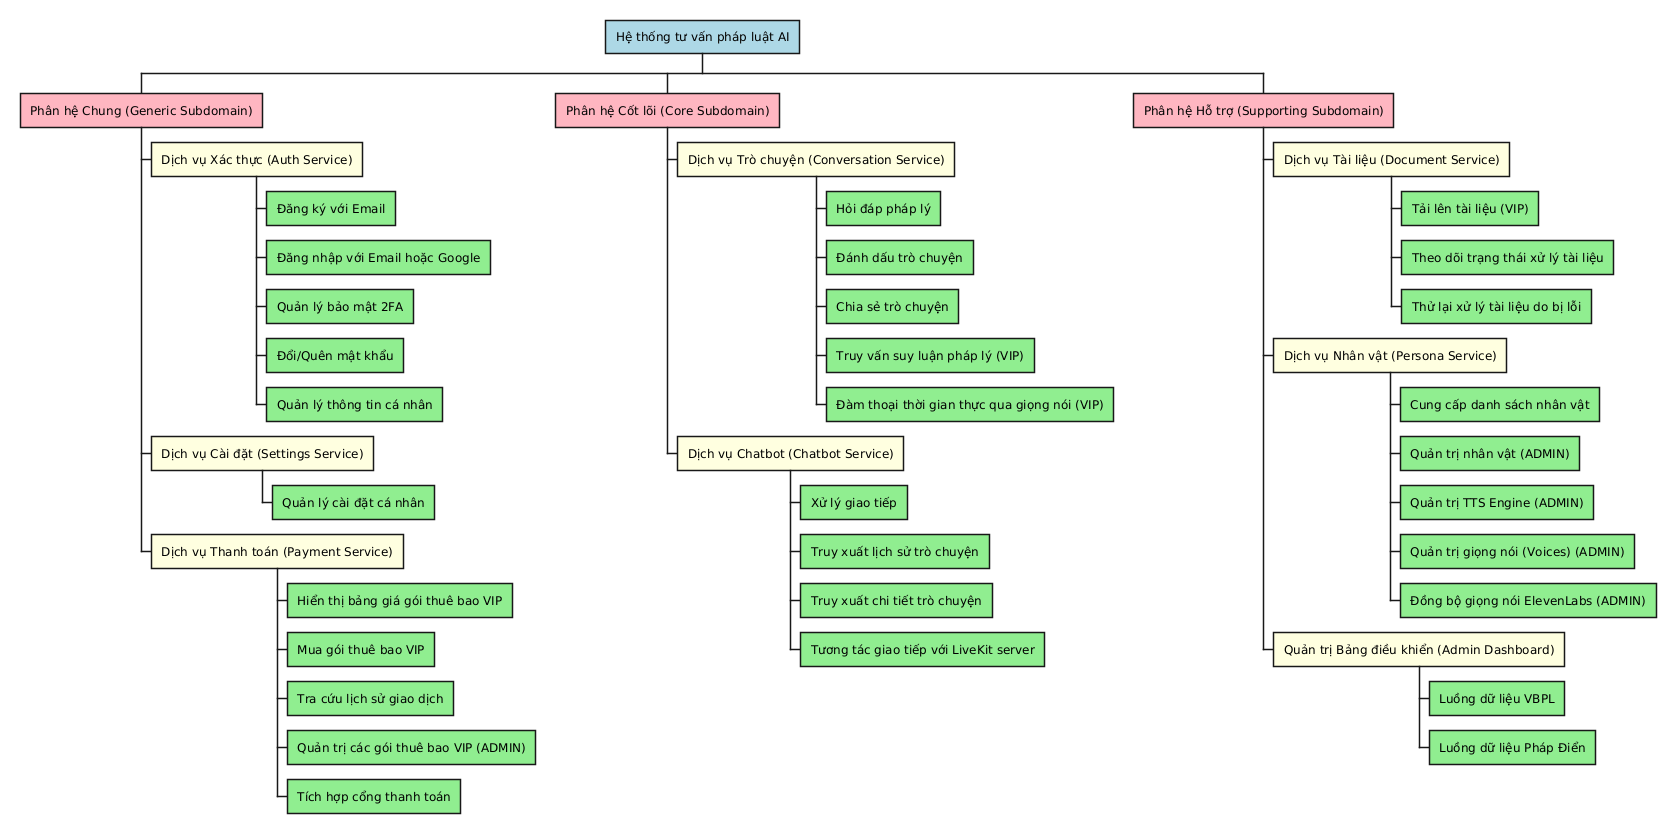
\includegraphics[scale = 0.25]{pictures/BFD.png}
\caption{Sơ đồ phân rã chức năng trong dự án}
\end{figure}
